
\documentclass[12pt]{report}         
\usepackage {utthesis2}              
\usepackage[utf8]{inputenc}
\usepackage{tocloft}
%\usepackage{ulem}
%\usepackage{setspace}
\usepackage[left=1.5in, right=1.5in]{geometry}
\usepackage{graphicx}
\usepackage[document]{ragged2e}
\usepackage{tabularx}
\usepackage{amsmath}
\usepackage{algorithm}
\usepackage{algorithmic}
\usepackage{ragged2e}
\usepackage{fancyhdr}
\usepackage{listings}
\pagestyle{plain}

\mastersthesis                     
\doublespace                   

\renewcommand{\thesisauthor}{Animesh Goyal}    %% Your official UT name.

\renewcommand{\thesismonth}{May}     %% Your month of graduation.

\renewcommand{\thesisyear}{2020}      %% Your year of graduation.

\renewcommand{\thesistitle}{Multi-Agent Deep Reinforcement Learning for RoboCup Rescue Simulator}     %% The title of your thesis; use
                                     %% mixed-case.

%\renewcommand{\thesisauthorpreviousdegrees}{Master of Science in Operation Research and Industrial Engineering}
                                     %% Your previous degrees, abbreviated;
                                     %% separate multiple degrees by commas.

\renewcommand{\thesissupervisor}{Peter Stone}
                                     %% Your thesis supervisor; use mixed-case
                                     %% and don't use any titles or degrees.

\renewcommand{\thesiscosupervisor}{Garrett Warnell}
                                     %% Your PhD. thesis co-supervisor; if any.
                                     %% Use mixed case and don't use any titles
                                     %% or degrees. Uncomment if you
                                     %% have a co-supervisor.
                                     %% (Ignored for Master's)



\renewcommand{\thesisauthoraddress}{4305 Duval St. 78751, Austin, TX, USA}
                                     %% Your permanent address; use "\\" for
                                     %% linebreaks.

\renewcommand{\thesisdedication}{...}
                                     %% Your dedication, if you have one; use
                                     %% "\\" for linebreaks.

%%%%%%%%%%%%%%%%%%%%%%%%%%%%%%%%%%%%%%%%%%%%%%%%%%%%%%%%%%%%%%%%%%%%%%%%%%%%%
%%%
%%% The following commands are all optional, but useful if your requirements
%%% are different from the default values in utthesis.sty.  To use them,
%%% simply uncomment (remove the leading %) the line(s).


\renewcommand{\thesisdegree}{Master of Science in Operation Research and Industrial Engineering } 

% \renewcommand{\thesisdegreeabbreviation}{...}
                                     %% Use this if you also use the above
                                     %% command; provide the OFFICIAL
                                     %% abbreviation of your thesis degree.

\renewcommand{\thesistype}{Master's Report}    %% Use this ONLY if your thesis type
                                     %% is NOT "Dissertation" for \phdthesis
                                     %% or "Thesis" for \mastersthesis.
                                     %% Provide the OFFICIAL type of the
                                     %% thesis; use mixed-case.

% \renewcommand{\thesistypist}{...}  %% Use this to specify the name of
                                     %% the thesis typist if it is anything
                                     %% other than "the author".

%%%
%%%%%%%%%%%%%%%%%%%%%%%%%%%%%%%%%%%%%%%%%%%%%%%%%%%%%%%%%%%%%%%%%%%%%%%%%%%%%

\begin{document}
\justify 
\noindent

\thesiscopyrightpage                 %% Generate the copyright page.

\thesiscertificationpage             %% Generate the PhD. certification page.

\thesistitlepage                     %% Generate the title page.

%\thesissignaturepage                %% Generate the Master's signature page.

\thesisdedicationpage                %% Generate the dedication page.


\begin{thesisacknowledgments}        %% Use this to write your
First and foremost I would like to thank my advisor, Peter Stone, for his guidance and encouragement throughout this report. He always made himself available to provide help and I could always count on his lightning-fast email responses. He gave me autonomy in finding a research topic and provided the right amount of guidance to help me make progress when I felt stuck. It has been a privilege to work with him. Garrett Warnell and Tsz-Chiu Au deserves a special thanks as collaborators and mentors throughout my research. They have provided invaluable help, especially with regards to their extensive reviews of my writing. Discussions with them have helped me flesh out ideas fully, and my writing and research ability have improved through their mentorship.    

I would like to thank several of my peers and colleagues for the help they’ve provided during my report. Aastha Goyal has provided invaluable input regarding the ..................

\end{thesisacknowledgments}          

\begin{thesisabstract}               

Recent advancement in the field of reinforcement learning has been driven on strategic games like Atari games, DOTA 2 and StarCraft where testing the model can be done quickly and in a safe manner. 

This work tries to explore strategic multi-agent games as an environment for deep reinforcement learning research. Large state space analysis and long term planning are one of the core requirements of strategic games in order to build a winning strategy. Building these winning strategies using deep reinforcement learning is a attractive as well as challenging task to work on specially when it incorporates multi-agent training where building the strategy is even more difficult. 

RoboCup Rescue Simulation Competition (RCRS), which is part of the annual RoboCup Competition, is an open source virtual environment that evaluates how effective multiple agents like ambulance team, police officer and fire brigades are in rescuing civilians and extinguishing fire from a city where an earthquake just happened. RCRS is challenging, easy to use and customize multi-agent scenario. 

In order to create RCRS environment where reinforcement learning algorithms can be tested, RCRS-gym, an open-source OpenAI Gym environment was created. We tested various algorithms for different map settings. 

Using Deep Q-Network and Proximal Policy Optimization algorithm, two agents (fire brigades) were able to learn how to extinguish fire in a city with 37 buildings (Small Map). The agents were able to understand the buildings where fire should be first extinguished so that it doesn't spread to other parts of the city quickly. This proves that the environment is suitable for developing a multi-agent deep reinforcement learning model. Another map having 100 buildings was trained using four fire brigades but required more training time and better hyperparameter tuning to make conclusions on the final performance.   
                                
\end{thesisabstract}                 

\tableofcontents                     

\newpage

\addcontentsline{toc}{chapter}{\numberline{}List of Figures}%
\listoffigures
\newpage
\addcontentsline{toc}{chapter}{\numberline{}List of Algorithms}%
\listofalgorithms
\newpage
\addcontentsline{toc}{chapter}{\numberline{}List of Tables}%
\listoftables
\newpage
% \listoftables      
% \newpage %% Uncomment this to generate list
%                                      %% of tables.
% \listofalgorithms    
% \newpage%% Uncomment this to generate list
%                                      %% of algorithms.
% \listoffigures        
% \newpage%% Uncomment this to generate list
                                     %% of figures.

\chapter{Introduction}            


On April 2019, OpenAI's DOTA 2 beat 99.4 percent of players in public matches \cite{dota2}. On October 2019, DeepMind's StarCraft II AI was able to play better than 99.8 percent of all humans \cite{Starcraft2}. These are milestone achievements where artificial intelligence has been used in the area of Multi Agent Systems (MAS). Although different techniques and algorithms were used in the above scenarios, in general, they are all a combination of techniques from two main areas: Reinforcement Learning and Deep Learning. 

Reinforcement learning (RL) is an area of machine learning where agents learn what actions to take in certain environment that results in higher cumulative reward over time. However, one of the drawbacks of RL is that the state space or action space can become too large to be completely known. This is where neural networks can be particularly useful as they are very good function approximators. Neural Networks can learn to map states to values, or state-action pairs to Q values. Rather than building a lookup table to store, index and update all possible states and their values, we can train a neural network on samples from the state or action space to learn to predict how valuable those are relative to our target in reinforcement learning. This is called Deep Reinforcement learning (DRL). 

\begin{figure}[!h]
    \centering
    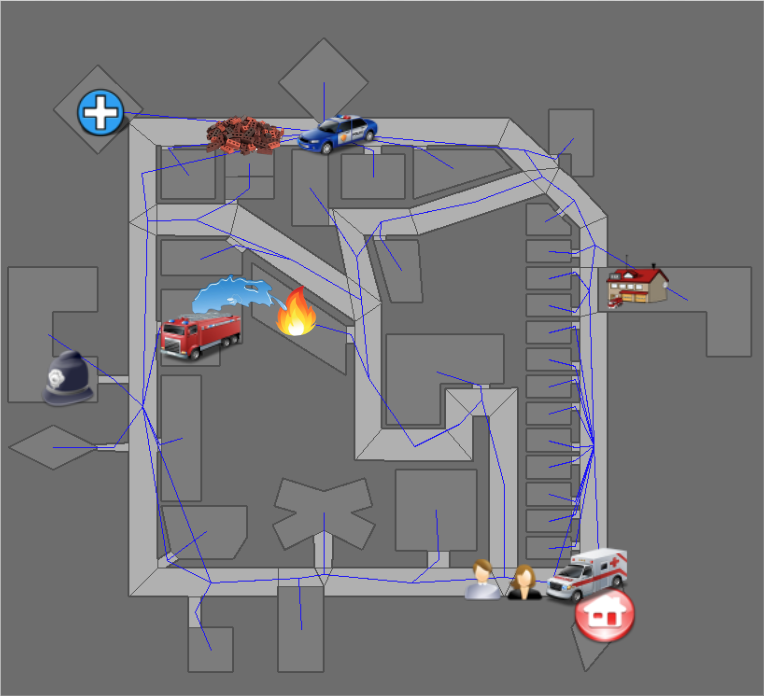
\includegraphics[width=12cm]{10.png}
    \caption{\textbf{RoboCup Rescue Simulation Environment:} RoboCup Rescue Simulator provides a 2D reinforcement learning environment where agents can be trained to save civilians and extinguish fire in a city where an earthquake has taken place}
    \label{fig:10}
\end{figure}

Together MAS and DRL are referred to as Multiagent Deep Reinforcement learning (MADRL). Currently, most of the work done in MADRL has been done in the field of video games (e.g. Atari games) and there is still a lot of work to be done for more realistic applications with complex dynamics, which are not necessarily vision based. 

One such domain is RoboCup Rescue Simulator (RCRS) (Figure ~\ref{fig:10}). RCRS is structured as a 2D discrete-time simulation system that depicts the situation after occurrence of earthquake in an urban area. Different agents like police officers, fire brigades and ambulance teams interact with the environment and with each other to accomplish tasks such as removing blockades, extinguishing fire and rescuing civilians. This task allocation can be handles in two ways: centralized or distributed. In centralized task allocation, a central agent manages all the agents and has the global knowledge whereas in case of distributed task allocation problem, each agent makes its own decisions and works only on its local information \cite{Nair}. 

\textbf{Contributions:} In this report, using centralized task allocation approach we have applied Deep Reinforcement Learning (DRL) algorithms to RCRS in order to train multiple fire brigades to extinguish the fire in the city on different sized maps having different number of agents and total buildings. The objectives are listed below as research questions: 

%%--------------Remove from here---------------------
% We compare a small map having 37 buildings and 2 fire brigades with a bigger map having 100 buildings and 4 fire brigades. The Deep Reinforcement learning techniques applied were Deep Q-learning (DQN) and Proximal Policy Optimization (PPO). Using DQN, \cite{mnih} was able to achieve human level performance on Atari games whereas PPO helped OpenAI's DOTA 2 team beat 99.4 percent of players in public match. 
%%--------------Remove from here---------------------

\begin{itemize}
    \item Is DRL appropriate for RoboCup Rescue Simulator?
    \item Can DRL learn a winning strategy for RCRS?
    \item If yes, what DRL algorithms are most suitable for it?
    \item What are the limitations of DRL model for RCRS?
    
    % \item \textbf{Built a RCRS-Gym interface, that can be utilized to apply various reinforcement learning algorithms to RCRS}
    % \item \textbf{Evaluated state-of-the-art reinforcement learning algorithms on RCRS, providing an extensive set of results for comparison}
    % \item \textbf{Showcased promising future research directions in this environment i.e. partial observability and including police officer and ambulance as the agent}
\end{itemize}

The rest of the report is structured as follows. Chapter 2 will help build important concepts that are important for understanding this project. Specifically it will explain the state-of-art DRL algorithms. In Chapter 3, detailed explanation of the simulator is done along with the state space, action space and reward function selected. In Chapter 4, implementation of the model in RCRS will be detailed along with the results. In Chapter 5, everything will be summarized and will discuss the future directions for the project. 


\chapter{Background}                       

This chapter will briefly cover the basic but very important concepts to understand the project like Reinforcement learning, Deep Reinforcement learning and Multi-agent system. With the definitions set, we will elaborate the work that is so far done to apply Reinforcement learning to RCRS. 

\section{Reinforcement learning}

Reinforcement learning is modeled as a Markov Decision process where the agent interacts with the environment to learn the actions in a certain state which would produce the highest reward. The reinforcement learning model is depicted in Figure ~\ref{fig:ReinforcementLearningModel} 

\begin{figure}[!h]
    \centering
    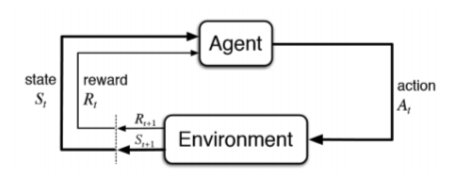
\includegraphics[width=12cm]{ReinforcementLearningModel.png}
    \caption{Abstract depiction of Reinforcement Learning Model: At some point in time t, the RL agent experiences a state $S_t$ and a reward $R_t$ for his action in time $t-1$. In state $S_t$, the agent takes action $A_t$ , for which the environment advances a time step, and the agent experiences a new state $S_{t+1}$ and a reward $R_{t+1}$ for action $A_{t+1}$}
    \label{fig:ReinforcementLearningModel}
\end{figure}

In order to maximize the long term reward signal, Reinforcement learning learns optimal actions for specific environment conditions by trial-and-error \cite{Barto}. 

At each time step t, the agent perceives a state $s_t$ in state space S from which it selects an action $a_t$ in the action space A by following a policy $\pi$. The agent receives a reward $r_t$ when it transitions to the state $s_{t+1}$ according to the environment dynamics, the reward function R($s_t$, $a_t$, $s_{t+1}$) and the transition function T($s_t$, $a_t$, $s_{t+1}$). Discount factor $\gamma$ $\in$ [0, 1] is applied to the future rewards. There are two types of RL approach: model based and model free. 

\textbf{Model based approach} uses a reduced number of interactions with the real environment during the learning phase. Its aim is to construct a model based on these interactions, and then use this model to simulate the further episodes, not in the real environment but by applying them to the constructed model and get the results returned by that model.

\textbf{Model free based approach} act in real environment in order to learn. The most common model-free technique is Q-Learning and Policy Gradient methods. 

\subsection{Q-learning} In Q-learning we are trying to build a Q-table Q(s,a) that stores all possible combinations of state s and action a. We sample an action a from the Q-table for the current state s. We observe the reward R and next state s'. Then from the Q-table we determine the next action a' in order to have maximum Q(s', a') (Figure ~\ref{fig:QLearning}). 

\begin{figure}[!h]
    \centering
    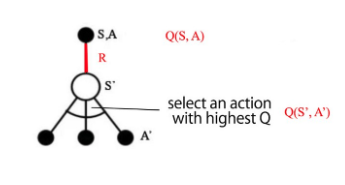
\includegraphics[width=8cm]{QLearning.png}
    \caption{Q-Learning working}
    \label{fig:QLearning}
\end{figure}

\[ Target = R(s,a,s') + \gamma max_{a'} Q_k (s', a') \] 

Here $\gamma$ is the discount factor who's value is between [0,1]. It controls the importance of future rewards vs the immediate ones. The lower the discount factor, the lesser important future rewards are and the agent will tend to focus on actions that will yield immediate rewards.    

\subsection{Policy Gradient} Policy gradient doesn't calculate the Q-value but instead uses a policy. 

\[ \pi_\theta (a | s) = P [ a | s ] \]

The policy learns a mapping from every state to action, and its objective is to find which actions lead to higher rewards and increase their probability. 

Policy gradient observes the environment and acts in it and keeps updating its policy based on the rewards it receives. 

\[ \tau = (s_1, u_1, s_2, u_2, ....., s_h, u_h ) \]

The objective function for policy gradient is:
\[ J(\theta) = E[\sum_{t=0}^{H} R(s_t, u_t); \pi_\theta] = \sum_{\tau} P(\tau;\theta) R(\tau) \] 

After multiple iterations, policy converges to a maximum value. Drawbacks of policy gradient method can be that it sometimes can get stuck in local maximum and will not be able to reach the global maximum.  

\section{Deep Reinforcement learning}

In situations where there is large state and action space, it is not feasible to learn the Q-values or a policy for each state and action pair. This is when Deep Reinforcement learning (DRL) is used where neural networks are utilized to model the components of RL. A representation of the architecture is given in Figure ~\ref{fig:DRLArchitecture}. 

\begin{figure}[!h]
    \centering
    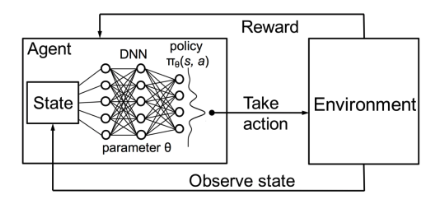
\includegraphics[width=12cm]{DRLArchitecture.png}
    \caption{Deep Reinforcement learning Architecture \cite{Mao}}
    \label{fig:DRLArchitecture}
\end{figure}


We consider two DRL model free based algorithms: Deep Q-Learning and Proximal Policy Optimization mainly because DQN showed great results on Atari games and helped the team achieve human level performance whereas using PPO, OpenAI's DOTA 2 team was able to beat 99.4 percent of players in a public match.  \\

\subsection{Deep Q-Networks(DQN)} DQN is a combination of Q-Learning and deep neural networks. DQN addresses the instabilities caused by using non-linear approximator to represent the Q-value by using two insights: experience replay and target network. 
Using Convolutional Neural Network (CNN) , DQN parameterizes an approximate value function Q(s, a; $\theta_i$) where $\theta_i$ are the weights of the network at iteration i. The experience replay stores the agent’s experiences $e_t$ = ($s_t$, $a_t$, $r_t$, $s_{t+1}$) at each time step t in a dataset $D_t$ = $e_1$,$e_t$ pooled over many episodes into a replay
memory. Then, mini batches of experience drawn uniformly at random from the dataset (s, a, r, s) $\sim$ U(D) are applied as Q-updates during the training. The
Q-learning update at iteration i follows the loss function:

\[ L_i (\theta_i) = E_{(s,a,r,s) \sim U(D) } [(r +  \gamma max_{a^{'}} Q(s^{'}, a^{'} ; \theta_i^{-}) - Q(s,a; \theta_{i}))^2] \]

\hfill \break
where $\theta_i$ are the Q-network parameters at iteration i and $\theta_i^{-}$  are the target network parameters. The target network parameters are updated with the Q network parameters every C steps and are held fixed between individual updates. \\

\subsection{Proximal Policy Optimization (PPO)} PPO is a type of policy gradient method which performs  comparably or better than state-of-the-art approaches while being much simpler to implement and tune. Careful tuning of the step size is required for achieving good results with policy gradient algorithms \cite{PPO}. Moreover, most policy gradient methods perform one gradient update per sampled trajectory and have high sample complexity. Schulman et al. \cite{Schulman} introduced PPO algorithm that solves both these problems. It uses a surrogate objective which is maximized while penalizing large changes to the policy. 
They defined a likelihood ratio 

\[ l_t(\theta) = \frac{\pi_\theta(a_t | s_t)}{\pi_{\theta old}(a_t | s_t)}\]

\hfill \break
PPO then optimizes the objective: 

\[ L^{CLIP} = \hat{E}_t [min(l_t(\theta) \hat{A}_t, clip(l_t (\theta) , 1- \epsilon , 1+\epsilon)\hat{A}_t)] \]

\hfill \break
where $\hat{A}_t$ is the generalized advantage estimate and $clip(l_t (\theta) , 1- \epsilon , 1+\epsilon)$ clips $l_t(\theta)$ in the interval [1 - $\epsilon$, 1 + $\epsilon$]. The algorithm alternates between sampling multiple trajectories from the policy and performing several epochs of SGD on the
sampled dataset to optimize this surrogate objective. Since the state value function is also simultaneously approximated, the error for the value function approximation is also added to the surrogate
objective to compute the complete objective function. 

\section{Multi-Agent Systems (MAS)}

In Multi-agents systems there are several agents that model each other's goals and actions \cite{Stone}. There may be direct communication between the agents in a fully general multiagent scenario. In multiagent systems, environment dynamics of other agents can be known by each agent which is unlike single agent systems, other agents can affect the environment in unpredictable ways and can create uncertainty in the domain. Therefore, multiagent systems can be viewed as having dynamic environments. Figure ~\ref{fig:MultiAgentSystem} shows a fully general multiagent scenario. 

\begin{figure}[!h]
    \centering
    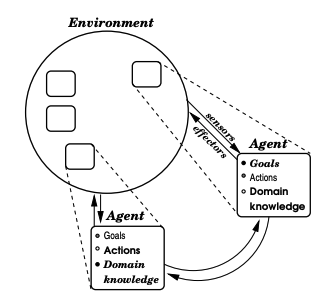
\includegraphics[width=12cm]{MultiAgentSystem.png}
    \caption{A fully general multiagent scenario. Agents can affect other agents actions, goals or domain knowledge or communicate directly with each other \cite{Stone}}
    \label{fig:MultiAgentSystem}
\end{figure}

\section{Multi-Agent Deep Reinforcement learning (MADRL)}

Since the success of deep RL using DQN proposed by \cite{Kavukcuoglu} many algorithms have been proposed to integrate deep learning to multiagent systems to solve complex problem in a variety of areas. This section provides a survey of these applications with a focus on the integration of deep learning and MARL. 

One of the earliest MADRL work was done by Tampuu et al \cite{Tampuu}. They had two independent DQN learning agents to play the Atari Pong game. They focused on building a reward function which resulted in either cooperative or competitive behaviours. Leibo et al. \cite{Leibo} studied about independent DQNs in the context of sequential social dilemmas which is a Markov game that satisfies certain inequalities. Their work focused on highlighting that cooperative or competitive behaviors exist not only as discrete actions but they are temporally extended over policies. Being able to capture sequential structure of real world social dilemmas, sequential social dilemma is an extension of matrix game social dilemma which has been previously applied to various phenomena in biology \cite{Cote}. DQN was used to find self interested independent learning agents to find equilibria of the sequential social dilemma which cannot be solved by the standard evolution methods used for matrix game social dilemma \cite{Weiner}. Lerer and Peysakhovich \cite{Lerer} were able to show theoretically and experimentally that agents can maintain cooperation using the famous Tit-for-Tat strategy for DRL (using function approximators). They used self play and two reward schemes: selfish and cooperative to construct the agents. Bansal et al. \cite{Bansal} used MuJoCo simulator to explore the emergent behaviors in competitive scenarios. They trained independent learning agents with PPO and incorporated two main modifications to deal with the Multiagent nature of the problem. Raghu et al. \cite{Raghu} studied how DRL algorithms like DQN, PPO performed in a two-player zero-sum games with tunable complexity called Erdos-Selfridge Spencer games. They were able to show that algorihms can exhibit wide variation in performance as the algorithms are tuned to the game's difficulty. Jiang and Lu \cite{Jiang} proposed a novel MADRL model that learns to communicate and exchange information while making decisions using actor-critic algorithm. Another interesting work in the field of MADRL was by Shao et al. \cite{Shao} for the game of StarCraft. In order to balance the units moved and attack strength of the enemy, they used parameter sharing multi-agent gradient descent SARSA algorithm using neural network to approximate the value function and reward function. However, high computation power was required for the implementation. 

\section{Reinforcement learning for RCRS}

On January 17th 1995, the Great Hanshin earthquake hit the Japanese port city Kobe with a magnitude of 6.8 on richter scale causing mass destruction taking approximately 7000 lives \cite{Bilski} \cite{RoboCup}. In response to the disaster, it was decided that the current disaster management policies should be changed. On April 30th 1999, RoboCup Rescue league was founded in order to promote international research towards the development of better rescue capabilities \cite{Bilski}.   

Over the years many teams have participated in the annual RoboCup Rescue league which consists of three competitions: robotics competition, virtual robot competition and the simulated agent competition. We will be focusing on the simulated agent competition known as RoboCup Rescue Simulation (RCRS) which is a perfect example of multiagent systems. 

In this section we will go over the work done by previous participating teams and how they have applied Reinforcement learning to RCRS. 

Martinez et. al \cite{Martinez} were the first one to implement Reinforcement Learning to RCRS. They introduced evolutionary reinforcement learning to improve the ambulance decision making process such as deciding the number of ambulances required to rescue a buried civilian. Their trained agent was able to outperform the participants of 2004 RCRS competition and was also computationally efficient. Visser et. al \cite{Visser2018RoboCupRS} developed a new framework to incorporate state-of-the-art machine learning algorithms into RoboCup Rescue competition code using the MATLAB Engine API for Java. They showed how supervised machine learning methods like classification and regression can be applied to assess the strategies of the agents and found the most relevant predictors. For example, estimating the chance of survival for a trapped civilian by predicting the remaining health point at the end of the scenario. Abdolmaleki et. al \cite{abdolmaleki} used SARSA to train the agent. They also proposed lesson-by-lesson learning which solved the problem of huge search space. Their proposed model increased the speed of learning and utilized very low memory. They discussed how temporal difference (TD) learning can be used to find the optimum policy for fire extinguishing tasks of a group of firefighter agents. Bitaghsir et. al \cite{Bitaghsir} introduced a layered neuro-fuzzy paradigm which is inspired from incremental learning. The paradigm was used for developing intelligent firefighter robots which involved layering increasingly complex learned behaviors. Aghazadeh et. al \cite{Aghazadeh} used parametric reinforcement learning to improve police force's decision making in RCRS. Using linear function approximator, they were able to perform the tasks using very less space. The work done till now has been quite intriguing but none of it involved MADRL to train the agents. This is what inspired us to write this report. 

\chapter{Modeling DRL for RCRS}

\section{Domain Description}

The competition is based on a complex simulation platform representing a city after a disaster. In order to make the simulator as realistic as possible, its designed to have heterogeneous agents (different types of agent), limited reach (agents can only perform tasks occurring close to them), random fire spread, injured victims, agents having limited communication with messages often getting dropped, agents being only able to see a short distance. It is therefore considered as a multiagent simulator \cite{Kitano}.  

RCRS has 3 major parts: Environment, Agents and Line of Sight:

\subsection{Environment}

The environment in RCRS comprises of various kinds of entities. The most important are buildings, roads, blockages, refuges and humans \cite{Morimoto}. 


\textbf{Buildings} are real constructions and have properties like area, fieryness and temperature, if its made of wood or cement. This information is useful for the simulator to calculate fire spread and building collapses. In case the building area is high and made of wood, fire will spread quickly. Simulator also changes the color of the building depending on the temperature and fieryness value. In case the both the properties are high, color gets darker and eventually turning black if the building is burned out. Note that fieryness value means how strong the fire is. 

\textbf{Roads} help the agents to move along the map. Some of the properties of roads are length, number of lanes. If a road is blocked due to agents standing in front or blockages, its not possible to move along it. 

\textbf{Blockages} is the property of blocking the lanes which usually occurs because of debris falling on the roads after earthquake. This prohibits agents to move forward. The only agent that can clear these blockages is police officers. They have a property of repair cost which lets the police officer know how difficult it is to clear them. 

\textbf{Refuge} are buildings where Fire Brigades can refill their water tanks and civilians can be kept safely. These buildings do not catch fire or collapse. 

\subsection{Agents} There are 3 kinds of agents in RCRS. 

\textbf{Fire Brigades} These agents are responsible for extinguishing fires in the buildings. They have water tanks with certain water capacity that needs to refilled from the refuge. Fire Brigades also have health points that decreases in case they catch fire or enter a building on fire. In case there health points drops to zero, they are considered dead. 

\textbf{Ambulance Teams} These agents are responsible for rescuing the injured civilians and carrying them safely to the refuge. They also have health points that decreases in case they catch fire. They cannot carry more than one victim at a time. 

\textbf{Police Officers} These agents are responsible to clear the blockages and allow other agents to complete their tasks. To clear a blockage, police officers need to get close to it. 

\subsection{Line of Sight} Each agent has a particular line of sight beyond which they cannot see. Since at each timestep, agents are able to visualize only a set of entities.

\hfill

In this report, we have focused on training multiple fire brigades to extinguish the fire as quickly as possible. Figure ~\ref{fig:RepresentationofSimulator} gives a visual representation of how the simulator looks. 

\begin{figure}[!h]
    \centering
    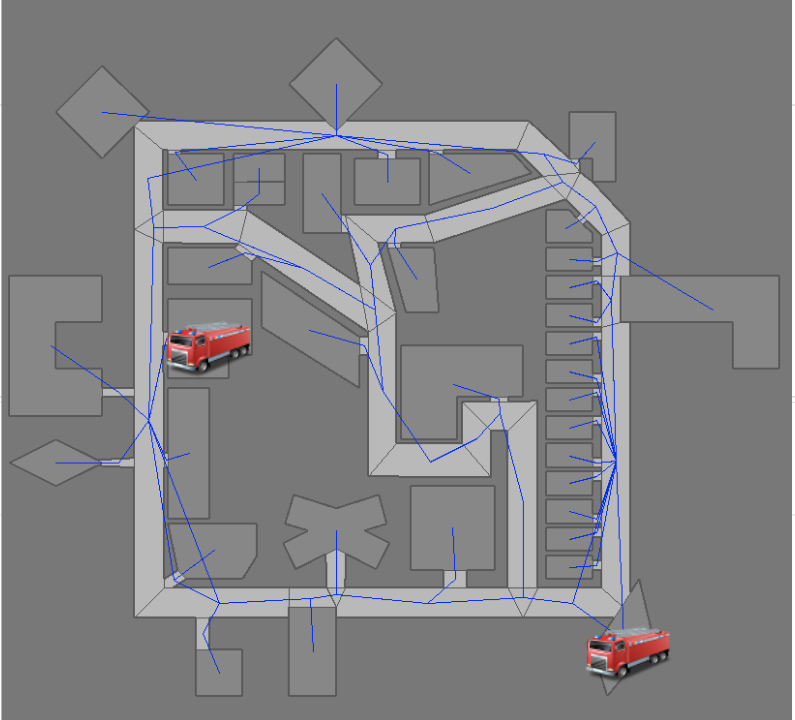
\includegraphics[width=12cm]{12}
    \caption{\textbf{Representation of the Simulator:} RoboCup Rescue Simulator with fire brigades. Different polygons are the buildings in the map. Grey color shows building is unburnt, yellow and red color shows building is burning, blue color depicts fire is extinguished and black shows the building is totally burnt. Note that as the shades get darker, building temperature and fieryness (degree of fire) increases.}
    \label{fig:RepresentationofSimulator}
\end{figure}

%---------------------------Put this in gym section ---------------------------------------------
In order to train the agents, we have taken help of Open AI's Gym toolkit \cite{brockman2016openai} which has been used to develop and compare different reinforcement learning algorithms. Reinforcement learning requires an agent and an environment. Environment, that represents the outside world to the agent and an agent that takes actions, receives observations from the environment which consists of a reward for the actions taken and knowledge of the new state. That reward implies how good or bad the action was, and the observation implies what will be the next state in the environment. Figure ~\ref{fig:23} explains how this loop is implemented to RCRS. 
%---------------------------Put this in gym section ---------------------------------------------

\begin{figure}[!h]
    \centering
    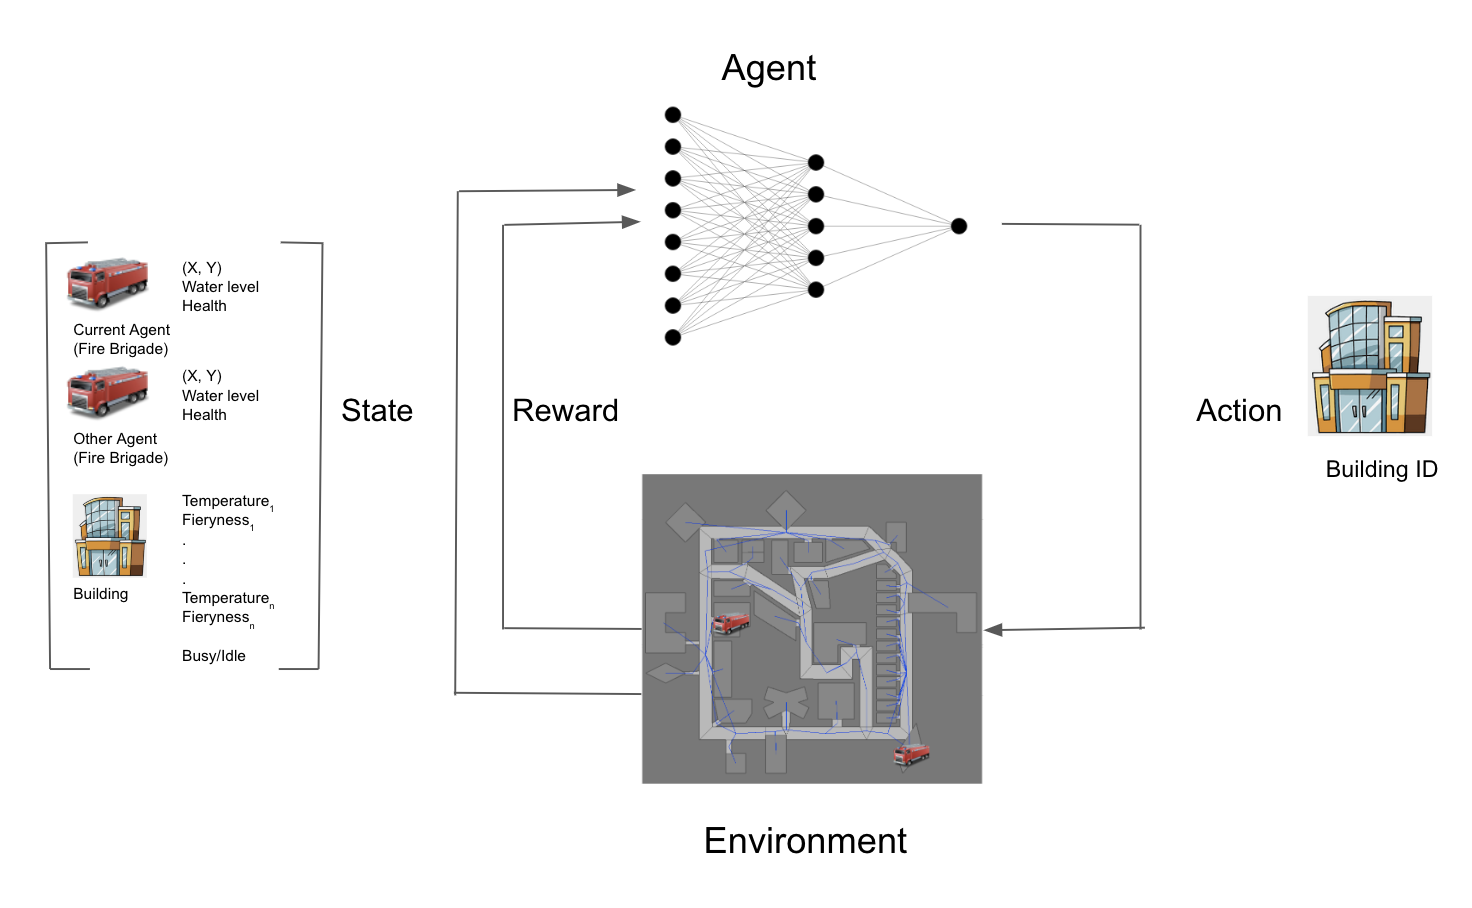
\includegraphics[width=12cm]{23}
    \caption{The neural network takes in state information and the reward collected at every timestep from the environment. State information contains (X,Y) coordinates, water level, health of the all the agents and temperature, fieryness of the buildings present. The neural network processes this information and outputs a building ID where the fire brigade needs to move next}
    \label{fig:23}
\end{figure}

Fire is initiated randomly following a Poisson distribution on the map. Fire brigades start searching the map looking for fire spots in the environment. Once the fire trucks detect a fire, they start extinguishing it. Note that extinguishing only takes place if the fire trucks are in a close proximity to the building. Fire brigades extinguish the fire until one of the three conditions hold true: (i) It is able to extinguish the fire completely, (ii) building has been completely burned out, or (iii) water in the fire tank is empty. For the first two situations, fire brigades start searching for a new building. For the third case, fire brigades move to the refuge to refill their tanks. In case the fire brigade sees more than one building on fire, it selects the one with highest priority using the following equation: 

\[ Priority = (\frac{Fieryness}{Total Area}) + (\frac{1}{\sqrt{distance}}) + {UnBurnedNeighbors}  \]

By this formula, priority is given to the building which has the highest fieryness, nearby and has the most number of neighbors.

Pseudo code for the algorithm that fire brigade follows is described in Pseudo-Algorithm 1.

\begin{algorithm}
\caption{Fire Brigade}
\begin{algorithmic}

\IF {(agent is inside refuge) and (water capacity of the fire truck is not full)}
\STATE  Refill the tank
\ENDIF 
\IF {(agent is stuck in blockage) or (building is not reachable)}
\STATE Search for buildings
\ENDIF
\IF {Water tank gets empty}
\STATE Start moving to the refuge
\ENDIF
\IF {(agent has not target)}
\IF {(agent sees a fire)}
\STATE Select target
\ELSIF {(communication is enabled)}
\STATE Request target
\ELSE 
\STATE  Search for buildings 
\ENDIF 
\ENDIF
\IF {(Target is not visible)}
\STATE Start moving towards the target
\ENDIF
\IF {(Target is visible)}
\STATE Extinguish fire
\ENDIF
\end{algorithmic}
\end{algorithm}


%---------------------------Put this in gym section ---------------------------------------------
At the starting of the simulation, a random building ID is provided to the Fire Brigade. After reaching its destination, the state information and the reward value is calculated and fed to the neural network which then outputs a vector of length equal to the number of building ID's. This vector is then passed through a softmax layer and then an Argmax layer which eventually gives the ID of the building to be visited next by our agent. 

%-------------------------------------------------------------------------------------------------

\section{Defining State Space, Action Space and Reward function}

The first step in applying reinforcement learning algorithms involves defining state space, action space and reward function. 

\subsection{State Space}
    
State space has three parts. The first part is the building information which consists of the temperature and fieryness. Note that, fieryness is a parameter to measure the degree of fire in a building. The second part is the agent information which gives the location ((X,Y) coordinates), water in the fire tanks and the health points of the fire brigade at each timestep. The third part is the busy/idle information which is a binary variable. Fire brigades receive a building id at each timestep as their target location. But it sometimes takes more than one timestep for them to reach the building. In the meanwhile, actions are being sent continuously. Hence, fire brigades have to ignore the actions till the time they visit the building they have been told to visit in the previous timestep. This information is passed over as a state information which will be highly valuable for our algorithm to perform better. Whenever the actions that are sent by the algorithm are used in the simulator (busy), 1 is sent back as the state information otherwise 0 is sent (idle). All the other state information values have certain ranges which are elaborated in Table ~\ref{table:StateInfoTable}. 

    \begin{table} [!h]
    \begin{center}
    \begin{tabular}{ l|l|l } 
    \hline
    State & Parameter & Range \\
    \hline \hline
    \multirow Building Information & Temperature of Building  & 0-100 \\ 
    & Fieryness of Building  & 0-10 \\ 
    
    \multirow Agent Information & (X, Y) Coordinates & 0-10000 \\ 
    & Water Level  & 0-15000 \\ 
    & Health Points & 0-10000 \\
    
    \multirow Busy/idle Information & Binary variable & 0/1 \\ 
    \hline
    \end{tabular}
    \caption{Ranges for values}
    \label{table:StateInfoTable}
    \end{center}
    \end{table}

\subsection{Action Space} 
    
The only action available to our agent is to move to the building which is on fire and therefore the action space consists of the ID's of the buildings. Note that extinguishing fire and refilling water are default characteristics of our agent i.e. whenever our agent is near a building on fire, it will try to extinguish it and whenever it is out of water, it will move to the refuge to refill the tank. Therefore these actions are not included in the action space. Detailed information about how the actions are performed as described in section 4.
    
\subsection{Reward Function}
        
Since the ultimate goal of the fire brigades is to extinguish fire as quickly as possible, we created a reward function that awards the agents higher rewards for keeping the fire to a minimum and penalize them if the fire increases. Fieryness is one parameter that measures the degree of burn in the building and hence keeping the overall fieryness value to a minimum results in a higher cumulative reward. Table ~\ref{table:RewardsTable} shows the reward function used in our case study. Table ~\ref{table:FierynessSeverity} shows the severity of the fieryness value. 
     
\begin{table} [!h]
\begin{center}
 \begin{tabular}{l | l} 
 \hline
 Fieryness Value & Reward Value  \\ [0.5ex] 
 \hline\hline
 0-2 & +10 \\
 3-5 & -5\\
 6-10 & -10  \\ 
 \hline
\end{tabular}
\caption{Reward Calculation}
\label{table:RewardsTable}
\end{center}
\end{table}
 
 
\begin{table} [!h]
\begin{center}
 \begin{tabular}{l | l} 
 \hline
 Fieryness Value & Severity  \\ [0.5ex] 
 \hline\hline
 0-2 & Slightly burned \\
 3-5 & Moderately burned\\
 6-8 & Critically burned\\ 
 9-10 & Totally burned\\
 \hline
\end{tabular}
\caption{Fieryness severity}
\label{table:FierynessSeverity}
\end{center}
\end{table}

\section{Model Architecture}

We use DQN and PPO architecture with a few modifications. We do not have the set of convolutional layers since the input to the neural networks is not an image. The input to the network is state representation and there is a separate output unit for each possible action. Different architectures were used for small map and big map which are mentioned in the following sections. 

\subsection{Model Architecture for Small Map} The 3 layer neural network consists of two fully connected (FC) layers having 64 units each (Figure ~\ref{fig:27}). It is followed by a softmax layer. The output layer is a fully connected linear layer with single output for each possible action. Every agent has its own neural network copy in order to allow it to learn its own local policy since every agent is trained independently. Note that environment here is fully observable. 

\begin{figure}[!h]
    \centering
    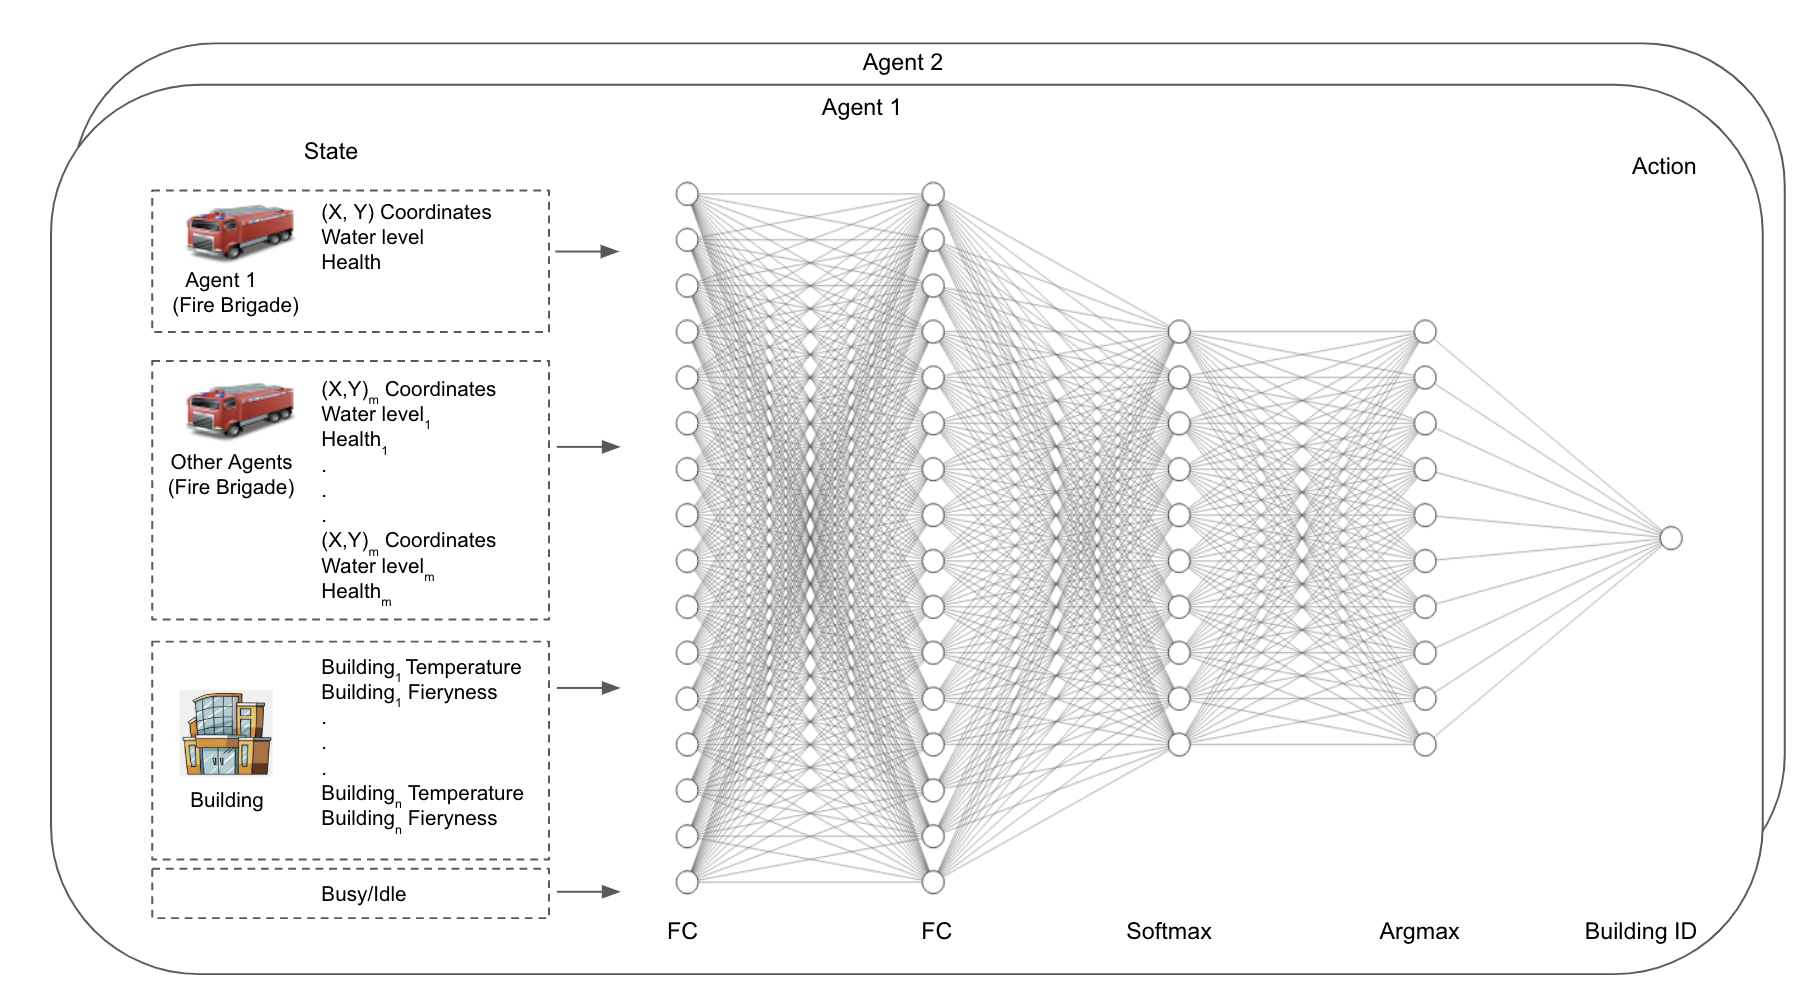
\includegraphics[width=14cm]{27}
    \caption{\textbf{Schematic Illustration of the Neural Network:} The input to the neural network is the state information which consists of a vector of length 94 having agent 1's current (X, Y) coordinates, water level, health, agent 2's current location, temperature, fieryness of the buildings and busy/idle condition. This is followed by 2 fully connected layers and a softmax and argmax layers to finally give a single action for the agent. The same architecture is used for second fire brigade also}
    \label{fig:27}
\end{figure}

\subsection{Model Architecture for Big Map} The 3 layer neural network consists of two fully connected (FC) layers having 64 units each (Figure ~\ref{fig:27}). It is followed by a softmax layer. The output layer is a fully connected linear layer with single output for each possible action. Every agent has its own neural network copy in order to allow it to learn its own local policy since every agent is trained independently. 

\begin{figure}[!h]
    \centering
    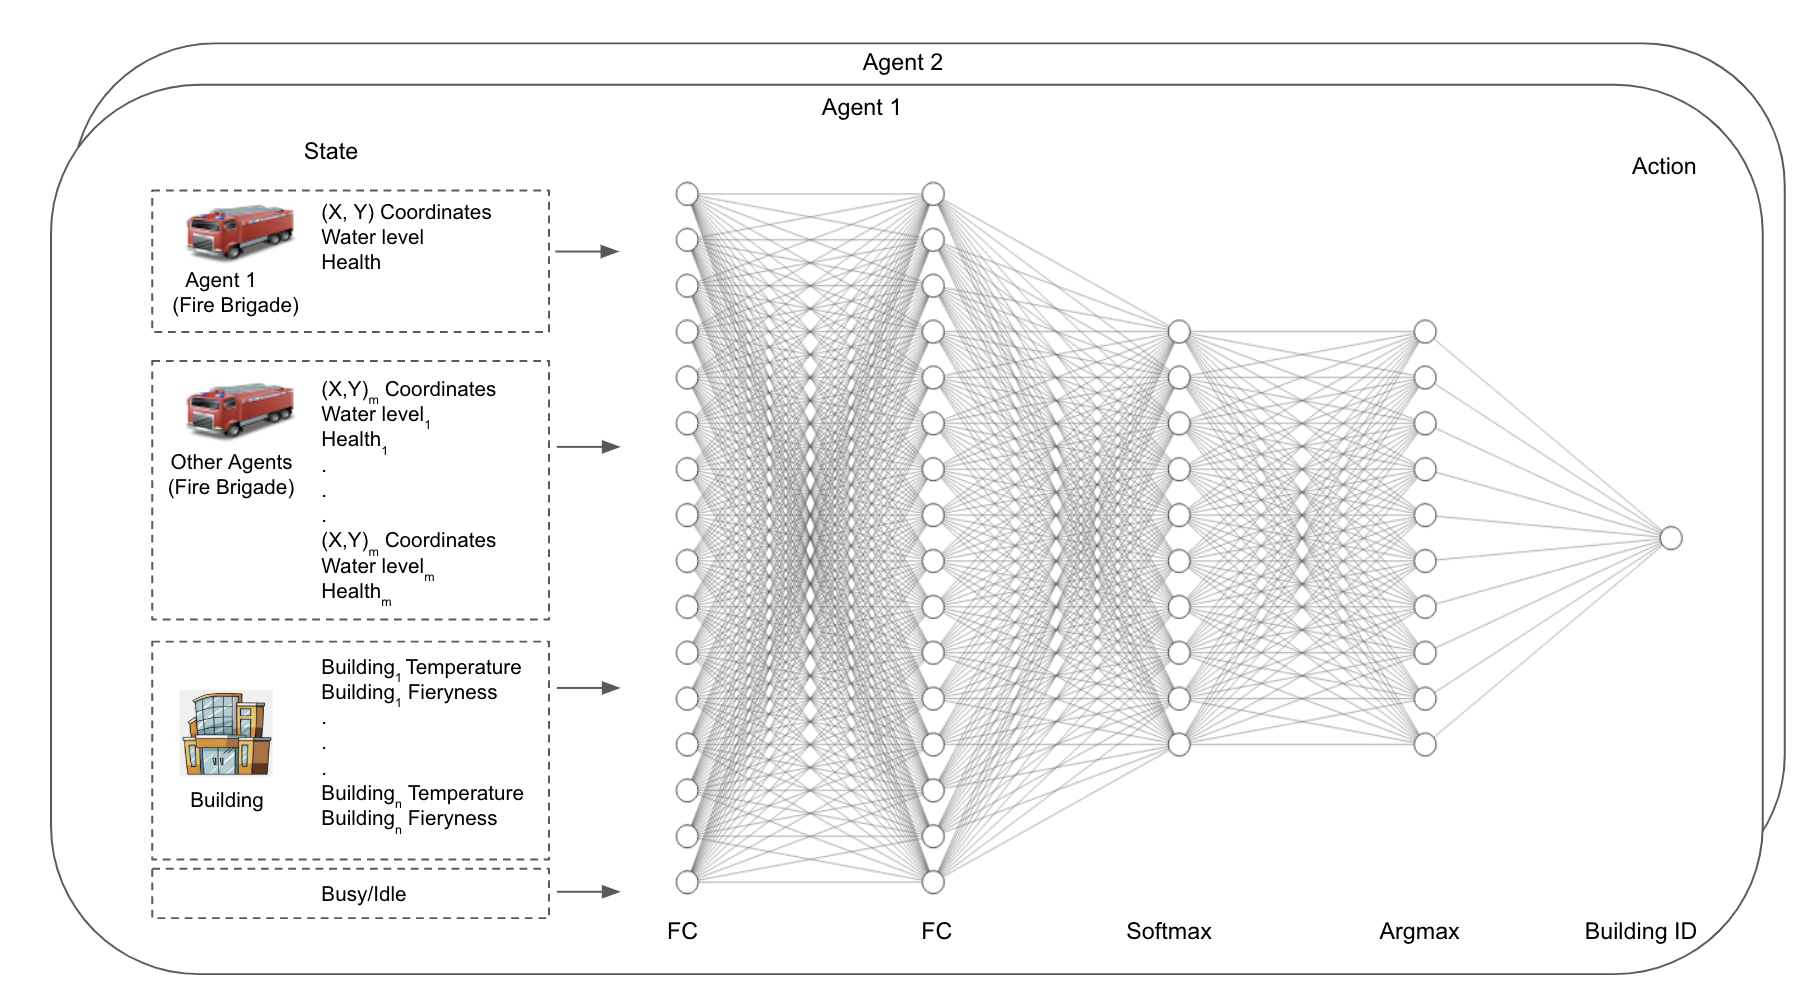
\includegraphics[width=14cm]{27}
    \caption{\textbf{Schematic Illustration of the Neural Network:} The input to the neural network is the state information which consists of a vector of length 94 having agent 1's current (X, Y) coordinates, water level, health, agent 2's current location, temperature, fieryness of the buildings and busy/idle condition. This is followed by 2 fully connected layers and a softmax and argmax layers to finally give a single action for the agent. The same architecture is used for second fire brigade also}
    \label{fig:27}
\end{figure}

\section{Hyperparameters}

\begin{table} [!h]
\begin{center}
 \begin{tabular}{l | l | l} 
 \hline
 Parameter & Small Map & Big Map  \\ [0.5ex] 
 \hline\hline
 Training Episodes & 1000 & 1000\\
 Testing Episodes & 1000 & 1000\\
 Discount factor ($\gamma$) & 0.99 & 0.99 \\ 
 Replay buffer size & 50000 & 50000\\
 Learning rate & 5e-4 & 5e-4\\
 Exploration $\epsilon$ & 1.0 $\rightarrow$ 0.02 & 1.0 $\rightarrow$ 0.02\\ 
 Exploration Fraction & 0.1 & 0.1\\
 Minibatch size B & 32 & 32\\
 Steps of the model before learning starts & 1000 & 1000\\
 Target network update frequency steps & 500 & 500\\
 \hline
\end{tabular}
\caption{Hyperparameters for DQN}
\label{table:x}
\end{center}
\end{table}

\begin{table} [!h]
\begin{center}
 \begin{tabular}{l | l | l} 
 \hline
 Parameter & Small Map & Big Map  \\ [0.5ex] 
 \hline\hline
 Training Episodes & 1000 & 1000\\
 Testing Episodes & 1000 & 1000\\
 Discount factor ($\gamma$) & 0.99 & 0.99 \\ 
 Replay buffer size & 50000 & 50000\\
 Learning rate & 5e-4 & 5e-4\\
 Exploration $\epsilon$ & 1.0 $\rightarrow$ 0.02 & 1.0 $\rightarrow$ 0.02\\ 
 Exploration Fraction & 0.1 & 0.1\\
 Minibatch size B & 32 & 32\\
 Steps of the model before learning starts & 1000 & 1000\\
 Target network update frequency steps & 500 & 500\\
 \hline
\end{tabular}
\caption{Hyperparameters for PPO}
\label{table:x}
\end{center}
\end{table}

\chapter{RCRS Gym Environment: Setup, Experiments, Analysis}

In order to implement the model introduced in Chapter 3 and prove its concepts, an OpenAI gym environment \cite{brockman2016openai} was created that allowed developing agents which are capable of extinguishing fire in the city. 

OpenAI is a framework that defines a standard structure that a DRL agent can be built with, that makes the structure of the agent easy to recognize by any developer and makes the agent compatible with any environment. 

Since OpenAI is built on Python, it can be easily connected with state-of-art DRL framework such as Tensorflow \cite{Abadi} with gym agents and use DRL techniques that use those frameworks provide. There are certain example algorithms available in OpenAI gym which simplifies the testing on a new environment. 

The proposed design is presented in Figure ~\ref{fig:OpenAIgymRCRS}. Section 4.1 elaborates about the setup that was created to adapt RCRS to allow the training of DRL agents. In Section ~\ref{Experiments}, experiments will be detailed and in Section ~\ref{Analysis}, results will be analyzed. 

\begin{figure}[!h]
    \centering
    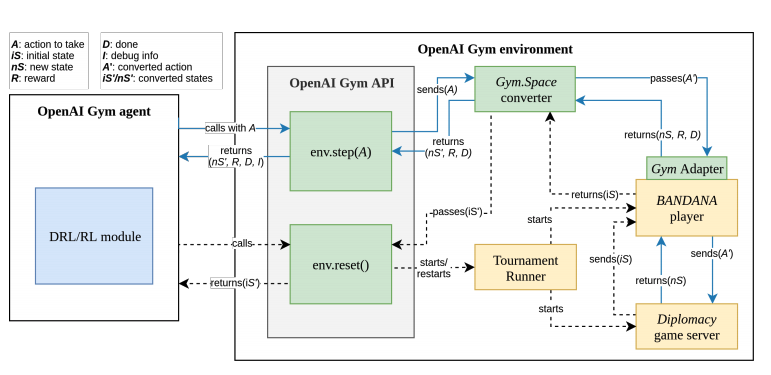
\includegraphics[width=14cm]{OpenAIgymRCRS.png}
    \caption{Conceptual model of the RCRS Gym environment and agent}
    \label{fig:OpenAIgymRCRS}
\end{figure}

\section{Setup} \label{Setup}

This section will deal with the process of building the environment and the logic behind the decision making process of RCRS. 

Section ~\ref{RCRSEnvironment} will describe the goal of the agent, what tasks will it perform after training, introduction to various maps and the complexity of the environment. 

Section ~\ref{OpenAIGym} will elaborate about gym framework and why it was chosen.

RCRS is written in Java and OpenAI gym in Python. There has to be a communication channel by which these two languages can communicate in order to send messages. Section ~\ref{CommunicationJavaPython} will discuss about how the communication between Java and Python was established. 

Finally, the overall implementation of RCRS-gym environment will be discussed in Section ~\ref{RCRSGymImplementation}. 

% Most of the Reinforcement learning algorithms are written in python. Since our aim is to build a simulator that is not only useful for our research work but can be used for future research by the community as well, we decided to integrate RCRS with gym that provides at easy-to-use suite of reinforcement learning tasks \cite{brockman2016openai}. Below is an example code that will run a random agent in our environment:
% \begin{lstlisting}

% import RCRS_gym
% import gym

% env = gym.make('RCRS-v2')
% env.reset()
% done = False
% while not done:
%     action = env.action_space.sample()
%     obs, rew, done, info = env.step(action)

% \end{lstlisting}

\subsection{RCRS Environment} \label{RCRSEnvironment}

%%%----------------Write Here Something---------------%%%

In order to test the algorithms, two maps were chosen. A "Small" map having fewer number of buildings and fire brigades to fasten the training process and a "Big" map having greater number of buildings and fire brigades. The Map specification can be seen in Table ~\ref{table:RCRSMapSpecs}. The representation of "Small" map can be seen in Figure ~\ref{fig:RepresentationofSimulator} and of "big" map in Figure ~\ref{fig:BigMap}

\begin{table} [!h]
\begin{center}
 \begin{tabular}{l | l | l} 
 \hline
 Map Name & Number of buildings & Number of Agents (Fire Brigades)  \\ [0.5ex] 
 \hline\hline
 Small & 37 & 2\\
 Big & 100 & 4\\
 \hline
\end{tabular}
\caption{RCRS Map Specifications}
\label{table:RCRSMapSpecs}
\end{center}
\end{table}

\begin{figure}[!h]
    \centering
    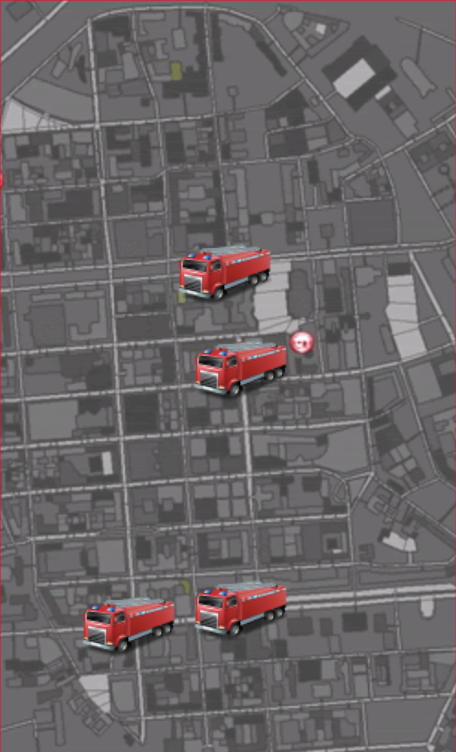
\includegraphics[width=8cm]{BigMap.png}
    \caption{Representation of "Big" Map}
    \label{fig:BigMap}
\end{figure}


\subsection{OpenAI Gym} \label{OpenAIGym}

OpenAI Gym defines a standard architecture that a reinforcement learning agent and the environment should have. Having a defined interface helps compare performance of different reinforcement learning algorithms in the same environment. 

OpenAI Gym maintains a repository, stable baselines \cite{stable-baselines}, having examples of implementations of state-of-art DRL methods. These implementations can be used to validate the environment. The defined gym interface is made of two methods that the agent will use to interact with the environment:

\begin{itemize}
    \item \emph{reset}: This function is used to reset the environment to its initial state and returns the initial observation. It is called whenever a new episode is started. 
    \item \emph{step}: This function receives the action that the agent wishes to use in order to interact with the environment as the argument and returns the observation, reward, done and info. 
    \begin{itemize}
        \item \emph{observation}: State of the environment
        \item \emph{reward}: Reward collected after the episode
        \item \emph{done}: returns true if episode is over
        \item\emph{info}: (optional) information value
    \end{itemize}
\end{itemize}

In addition to the above attributes, "action space" and "observation space" should be defined in order to abstract the environment to generic code. 

\begin{itemize}
    \item \emph{action space}: The space of possible actions that will be used to generate the actions
    \item \emph{observation space}: The space that defines the dimension of the environment's state
\end{itemize}





\subsection{Communication between Java and Python} \label{CommunicationJavaPython}

\subsection{RCRS-Gym Implementation} \label{RCRSGymImplementation}

\section{Experiments} \label{Experiments}

As mentioned in the Introduction section, we are comparing two maps having different number of buildings and fire brigades. The first map is having 37 buildings and 2 fire brigades. The results of running PPO, DQN is shown in the figure. 

\begin{figure}[!h]
    \centering
    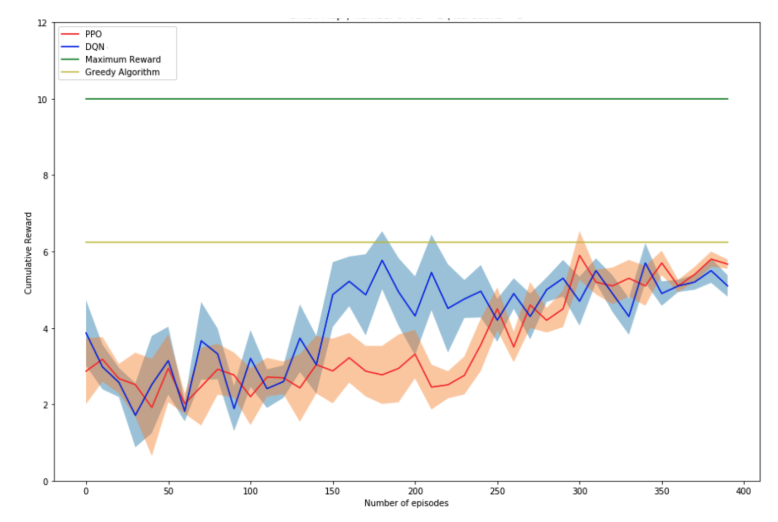
\includegraphics[width=12cm]{29.png}
    \caption{\textbf{Comparison of Results for Small Map}}
    \label{fig:x}
\end{figure}

\begin{figure}[!h]
    \centering
    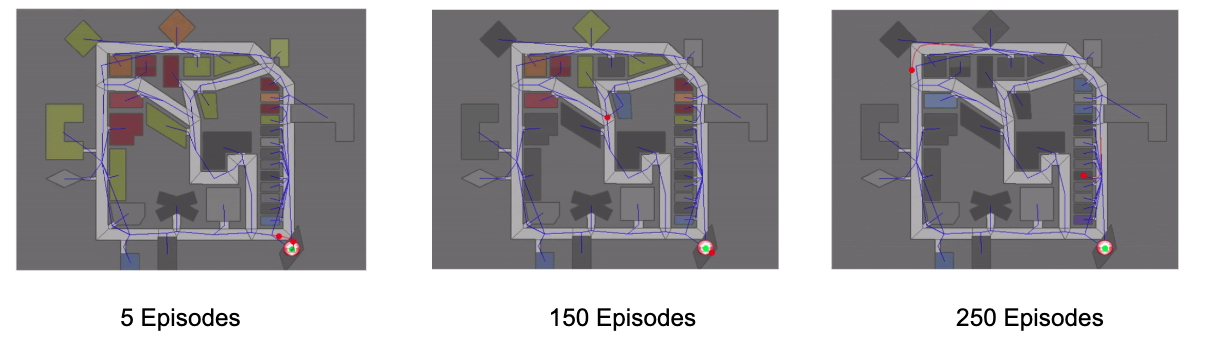
\includegraphics[width=16cm]{PPO.png}
    \caption{\textbf{Comparison of Results for Small Map}}
    \label{fig:x}
\end{figure}

\section{Analysis} \label{Analysis}

\begin{figure}[!h]
    \centering
    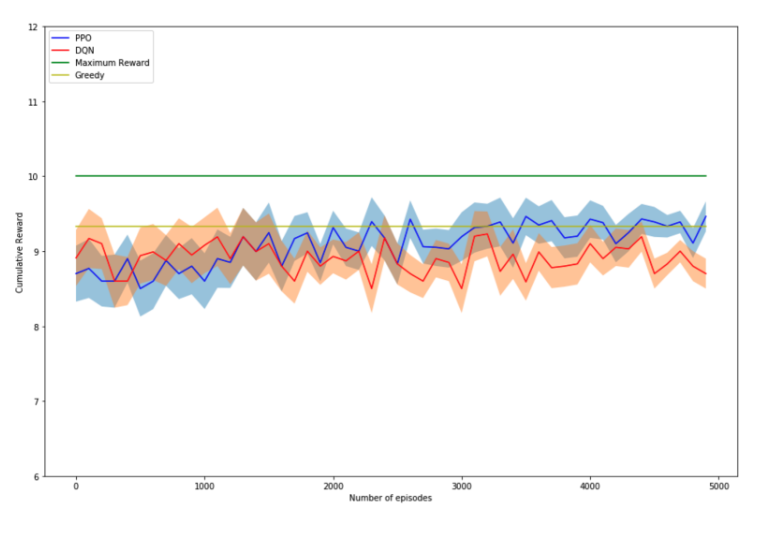
\includegraphics[width=12cm]{30.png}
    \caption{\textbf{Comparison of Results for Big Map}}
    \label{fig:x}
\end{figure}

\chapter{Conclusion and Future Work}
\appendix
\chapter{Plots}
\chapter{Tables}


%\addcontentsline {toc}{chapter}{Bibliography} 
                                     %% Force Bibliography to appear in contents

\bibliographystyle{plain}
\bibliography{bibliography.bib}      

\begin{thesisauthorvita}             
\end{thesisauthorvita}               

\end{document}                       %% Done.
